\documentclass[tikz,border=8pt]{standalone}
\usetikzlibrary{arrows.meta,positioning}
\begin{document}
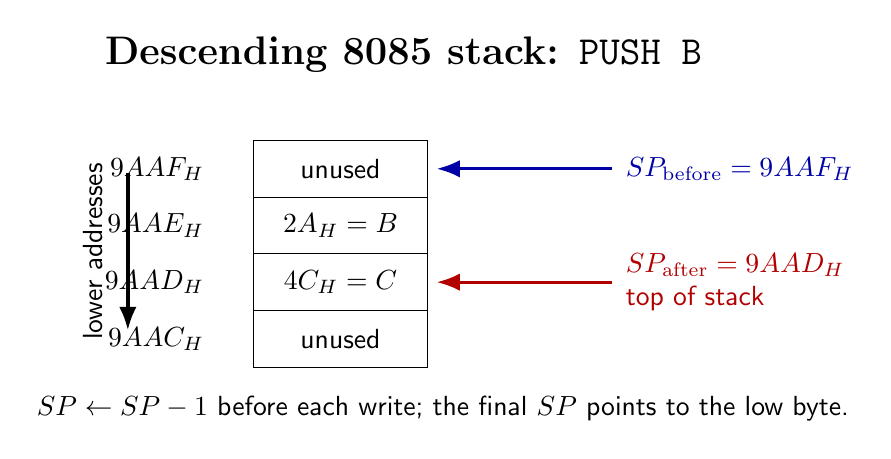
\begin{tikzpicture}[font=\sffamily,>=Latex,cell/.style={draw,minimum width=2.2cm,minimum height=.72cm},note/.style={align=left}]
\node[font=\Large\bfseries] at (4.5,5.05) {Descending 8085 stack: \texttt{PUSH B}};
\foreach \a/\y/\v in {9AAF/3.6/unused,9AAE/2.88/$2A_H=B$,9AAD/2.16/$4C_H=C$,9AAC/1.44/unused}{
  \node[cell] (m\a) at (3.7,\y) {\v};
  \node[left=5mm of m\a] {$\a_H$};
}
\draw[very thick,blue!65!black,->] (7.15,3.6)--(4.92,3.6);
\node[right,note,blue!65!black] at (7.2,3.6) {$SP_{\rm before}=9AAF_H$};
\draw[very thick,red!70!black,->] (7.15,2.16)--(4.92,2.16);
\node[right,note,red!70!black] at (7.2,2.16) {$SP_{\rm after}=9AAD_H$\\top of stack};
\draw[very thick,->] (1.0,3.55)--(1.0,1.55);
\node[rotate=90] at (.55,2.55) {lower addresses};
\node[note] at (5.0,.55) {$SP\leftarrow SP-1$ before each write; the final $SP$ points to the low byte.};
\end{tikzpicture}
\end{document}
